

\section{Case da Eletrônica Embarcada}
\label{case}

 
\begin{table}[ht!]

	\begin{tabular}{r l|l p{12cm} }
		
		\textcolor{gray}{Especificação} &&& 	{Case de Alumínio para a eletrônica
		embarcada}\\
		\textcolor{gray}{Data} &&& 				{03/03/2015}\\
        \textcolor{gray}{Beneficiado} &&&		{Speed Form Ind. Com. Ltda}
        \\
        \textcolor{gray}{CNPJ} &&& 				{27.497.726/0001-38} \\
        \textcolor{gray}{Número Nota} &&& 		{2395} \\
		\textcolor{gray}{Quantidade} &&& 		{1} \\
		\textcolor{gray}{Valor} &&& 			{R\$9.570,00} \\
		\textcolor{gray}{Data Sheet} &&& 		{-}
		\\

		\textcolor{gray}{Função no projeto} &&& {Case da eletrônica embarcada. Vaso de
		pressão para 50 m de profundidade. }
		\\
		\textcolor{gray}{Razão da Escolha} &&& {Menor prazo de entrega e empresa já
		conhecida pelo grupo.}
		\end{tabular}
\end{table}

\newpage
\subsection{Foto do Material}
\begin{figure}[H]
 \centering
 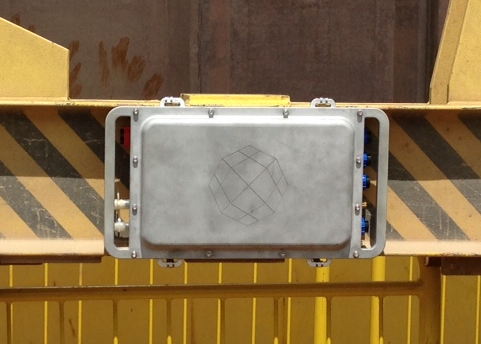
\includegraphics[width=1\columnwidth]{Case/foto.png}
 \caption{Case da eletrônica embarcada}  
\end{figure}

\subsection{Nota Fiscal}
\includepdf[pages=2,angle=-90]{Case/nota.pdf}